\section{Human Study Details.}

\begin{figure*}[t]
    \centering
    
    % ---- Top: 2D UI ----
    \begin{subfigure}{0.7\linewidth}
        \centering
        \includegraphics[width=\linewidth]{sec/images/2d_UI.jpg}
        \caption{\texttt{2D} survey interface. Participants see the prior ground truth, question text, and a numeric answer box, and can replay or scrub the video.}
        \label{fig:ui-2d}
    \end{subfigure}
    \vspace{0.6em}
    
    % ---- Bottom: 3D UI ----
    \begin{subfigure}{0.8\linewidth}
        \centering
        \includegraphics[width=\linewidth]{sec/images/3d_UI.jpg}
        \caption{\texttt{3D} survey interface. The layout mirrors the \texttt{2D} condition, with additional depth prior ground truth.}
        \label{fig:ui-3d}
    \end{subfigure}
    
    \caption{\textbf{Human study interface.}
    Example screenshots of the \texttt{2D} (top) and \texttt{3D} (bottom) survey UIs.
    Both interfaces present the physical prior, quantitative question, and a numeric input field, while allowing participants to replay and scrub the video timeline.}
    \label{fig:ui-overview}
\end{figure*}


To contextualize model performance and establish an empirical upper bound on human quantitative physical reasoning, we conducted a survey study using the Gorilla Experiment Builder platform. The platform supported video presentation, question randomization, and structured data collection. Below, we describe the participant cohort, task construction, interface design, evaluation methodology, and resulting performance trends.

\subsection{Participants}
Participants were recruited from a mix of undergraduate, graduate, and PhD researchers, including individuals with advanced training in various fields including engineering, physics, and mathematics. This allowed us to approximate both typical human performance and an expert-level upper bound. Participants were informed that they could freely choose their reasoning strategy---including intuitive estimation, visual approximation, or explicit calculation---in order to reflect natural human reasoning rather than enforce a prescribed computation protocol.

Our survey is divided into two versions: a \texttt{2D} survey and a \texttt{3D} survey. Both the \texttt{2D} and \texttt{3D} surveys were completed by multiple participants, including several with substantial technical backgrounds. A subset of participants completed both tasks, enabling direct cross-dimensional comparisons of individual consistency.

\subsection{Task Construction and Experimental Design}
Following the 36 fine-grained video categories defined in \autoref{subsec:video_type}, we organized the full dataset into these category units for both model and human evaluation. Each category contains a small pool of representative videos, from which stimuli were sampled during the experiment.

Participants were randomly assigned to either the \texttt{2D} survey or the \texttt{3D} survey. Each participant viewed 18 videos, one sampled per category within their assigned dimensionality. Each video was followed by 1--3 quantitative kinematic questions, with the same priors and task formulations used in our VLM evaluation (e.g., estimating acceleration magnitude, inferring relative size changes, or recovering object velocity).

The UI interface was intentionally designed to be concise and unobtrusive. For each trial, participants were presented with:
\begin{itemize}
\item A video with standard playback controls;
\item The physical prior ground truth (\texttt{A/S/V}) and/or corresponding depth information for \texttt{3D} videos;
\item The quantitative question texts;
\item Numeric input boxes (numbers only).
\end{itemize}

Participants could freely replay, pause, and scrub the video timeline. Scrubbing resolution was restricted to whole seconds to match the temporal information available to VLMs, which process videos solely as pixel sequences without access to exact timestamps. The interface permitted unrestricted video replay to minimize memory effects and ensure that both humans and VLMs operated over comparable visual evidence.

\begin{figure}[t]
    \centering
    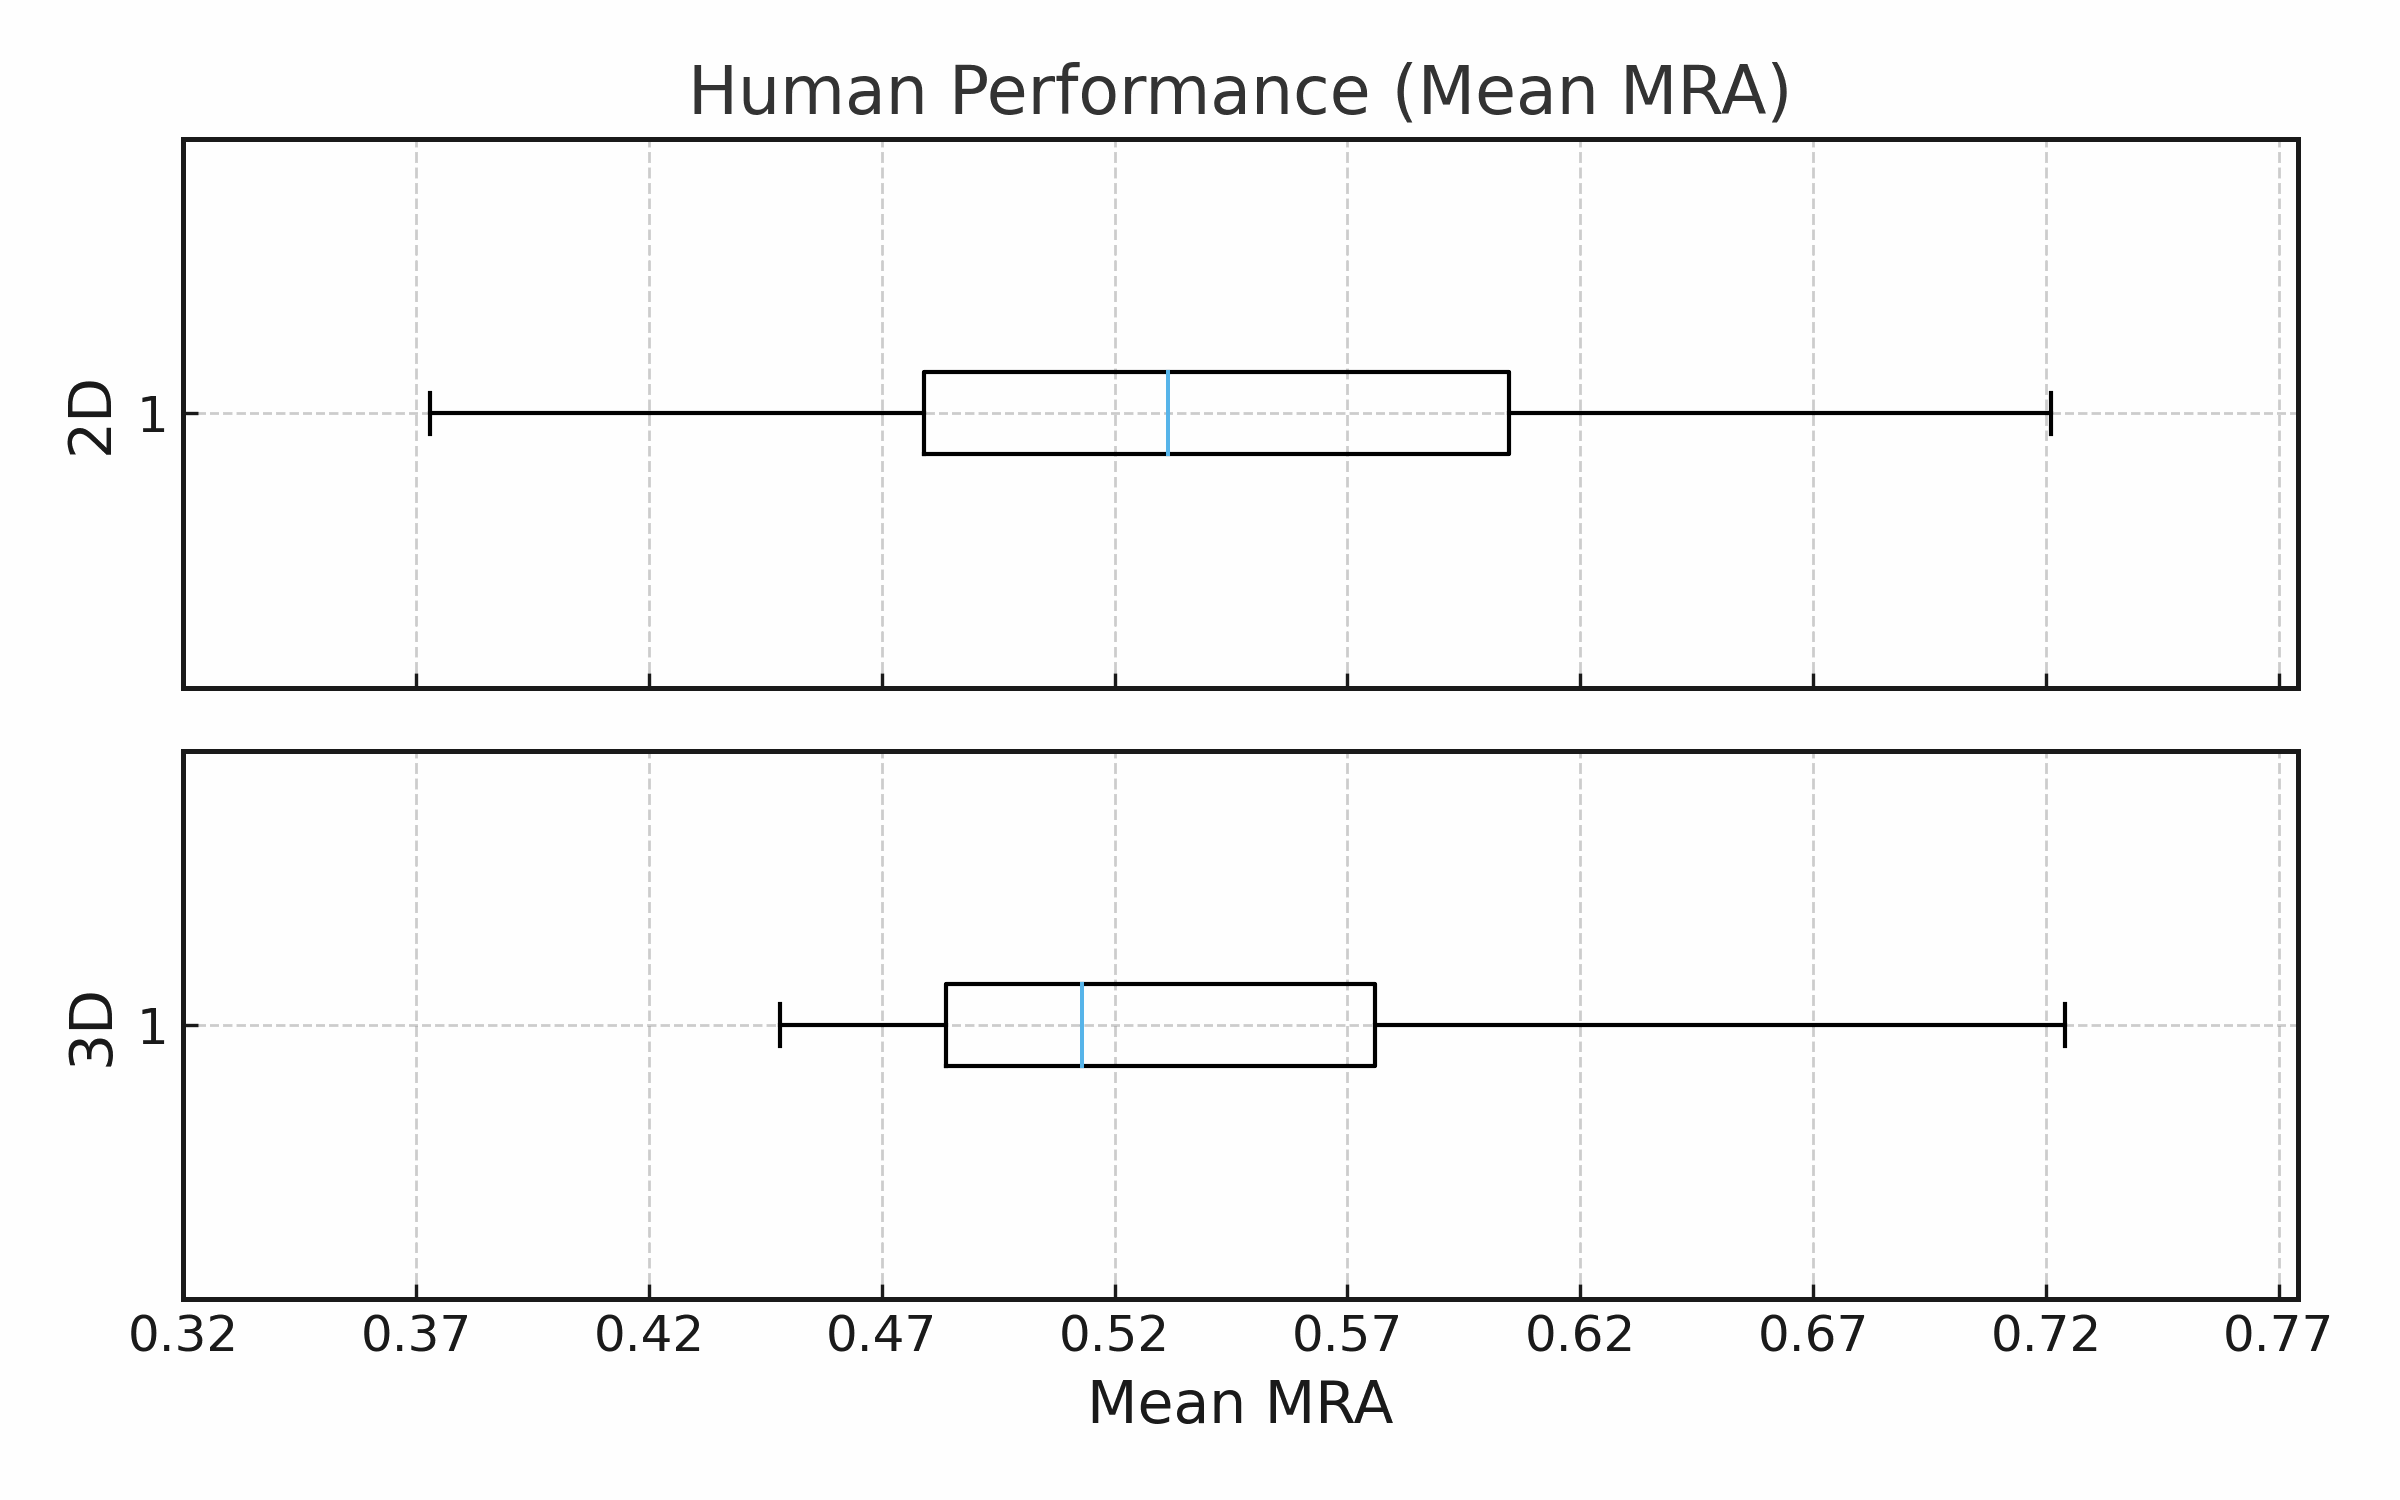
\includegraphics[width=0.95\linewidth]{sec/images/human_mra_boxplots.png}
    \caption{\textbf{Distribution of human quantitative reasoning performance.}
    Horizontal boxplots summarize participant-level mean MRA scores for the \texttt{2D} (top) 
    and \texttt{3D} (bottom) survey conditions.}
    \label{fig:human-boxplot}
\end{figure}

\subsection{Evaluation Metric}
Human responses were evaluated using the same MRA metric introduced in Section~\ref{sec:evaluation}. 
For each individual question, we compute MRA by averaging accuracy over ten relative-error tolerance thresholds, yielding a smooth, threshold-agnostic measure of quantitative precision. 
After computing an MRA score for every answered question, we aggregate performance at the participant level by taking the mean MRA across all questions completed by that participant. 
Figure~\ref{fig:human-boxplot} presents participants performance for the \texttt{2D} and \texttt{3D} surveys, respectively.


\subsection{Results and Observations}
We observe a few findings from the results.

\noindent\textbf{Strong cross-dimensional consistency.}
Across participants who completed both tasks, MRA scores for \texttt{2D} and \texttt{3D} surveys were highly correlated. High-performing participants in \texttt{2D} almost universally remained high-performing in \texttt{3D}, suggesting that human physical intuition is stable and transferrable across dimensional modalities.


\noindent\textbf{Human upper bound substantially exceeds VLM performance.}
Top human participants achieve MRA = \textbf{0.721} in \texttt{2D} and  MRA = \textbf{0.724} in \texttt{3D}, showing better performance than the evaluated VLMs. Although the average human performance is not higher than model performance, the human upper bound remains far above current VLM capabilities. This gap is particularly notable given the modest sample size of our study; even with limited data, humans exhibit strong physical reasoning competence that remains challenging for contemporary models.


\noindent\textbf{Practical implications.}
These findings indicate that while VLMs may approximate average-level human intuition in some settings, they remain far from achieving human-like precision or matching expert-level reasoning. The human study therefore provides a meaningful benchmark for assessing the gap between current VLM capabilities and the aspirational goal of physically grounded, human-level visual reasoning.

